\chapter{Introduction}
One of the biggest challenges in modern research is the study and the 
development of humanoid robots. Building a machine that is capable of executing 
the same tasks that the humans do is of fundamental importance for the future 
of our society, freeing people from dangerous and laborious jobs, increasing 
productivity and well-being. The idea of replicating the characteristics of 
the human body has fascinated humanity since the conception of Leonardo's
Robot (1495) by Leonardo Da Vinci \cite{Moran2007TheDaVinciRobot}. Human 
knowledge has advanced so much in the last centuries that the dream of 
building a machine that resembles the human body has finally become true.

This chapter introduces humanoid robots, giving an overview of the technology 
that has been developed in the last decades and a comparison to other robots
such as manipulators and unmanned ground vehicles. The problem of legged 
robot locomotion is then discussed, describing the current state-of-the-art 
research, the modules that allow a 
humanoid robot to safely move inside a specific environment, such as 
localization, mapping, planning and control, and the way they seamlessy work
together in order to realize humanoid gaits.

Even if humanoid robots are nowadays capable of realizing astonishing tasks,
many challenges are yet to be solved before their introduction in our 
society, making them part of our daily life. The goal of this thesis is that 
of studying humanoid robot locomotion in a world known as \textit{World of 
Stairs}, where the environment surrouding the robot is composed of 
horizontal patches located at different heights \cite{ECC19}. This chapter 
concludes by presenting an overview of the thesis, discussing its 
structure and the content of each chapter. 

\section{Humanoid Robots}
The development of humanoid robots started in 1967 with the WABOT-1
\cite{Kato1973TheWABOT1AI}, shown in Fig. \ref{fig:wabot-1}, created by Waseda
University. WABOT-1 is
the first anthropomorphic robot able to 
walk with its limbs and carry objects with its hands. It was also equipped with 
a vision and a communication system that allowed it to communicate with people 
in Japanese. The most famous humanoid robot is probabily ASIMO
\cite{Sakagami2002TheIntelligentASIMO}, developed by HONDA (Fig.
\ref{fig:asimo}). Its development started in the
1980s and it was preceded by many different version before being presented in
2000.
The last version of ASIMO is 130 cm tall and is able to recognize objects,
gestures, sounds and 
faces, making it able to interact with humans. It is equipped with multiple 
sensors such as laser and infrared that allow it to navigate autonomously. 
ASIMO is able to walk and run up to a speed of 9 km/h with an 
autonomy of one hour. Another very famous robot is NAO \cite{NAOdesign},
which development has been started by Aldebaran and continued by Softbank after 
its acquisition. NAO (Fig. \ref{fig:nao-v6}) is the official robot used in 
the RoboCup \cite{Kitano1997RoboCup} Standard Platform League, an international
competition that consists in a soccer tournament where the teams are composed 
of 5 robots. The goal of RoboCup is that of winning against a FIFA
World Cup winner team by 2050. Most recent and advanced humanoid robots 
includes iCub \cite{Sandini2007iCub}, shown in Fig. \ref{fig:iCub}, designed 
by the RoboCub Consortium and built by Italian Institute of Technology,
with the idea of being a research platform for cognitive robotics;
ATLAS (Fig. \ref{fig:atlas}), developed by Boston Dynamics for emergency service
and rescue operations, such as those described by DARPA Robotics Challenge
\cite{Atkenson2018DARPARoboticsChallengeFinals}, illustrated in Fig.
\ref{fig:drc}; Valkyrie (Fig. \ref{fig:valkyrie}), developed by NASA with the 
aim of advancing human spaceflight and extraterrestrial exploration
\cite{Radford2015Valkyrie}.

\begin{figure}
  \centering
  \begin{subfigure}[b]{0.4\textwidth}
    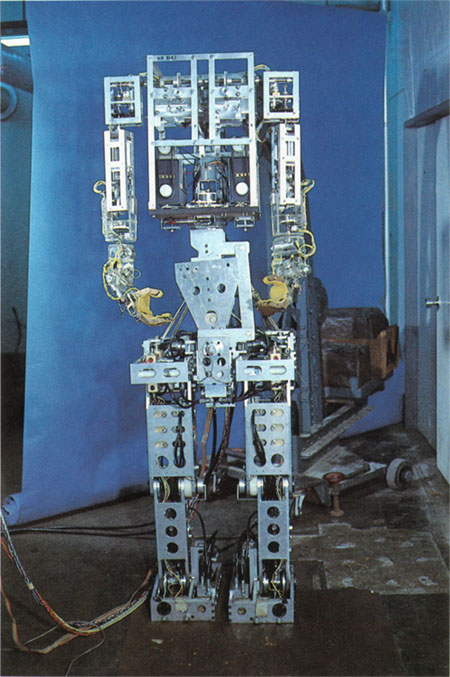
\includegraphics[width=\textwidth]{figures/WABOT-1.jpg}
    \caption{}
    \label{fig:wabot-1}
  \end{subfigure}
  \begin{subfigure}[b]{0.4\textwidth}
    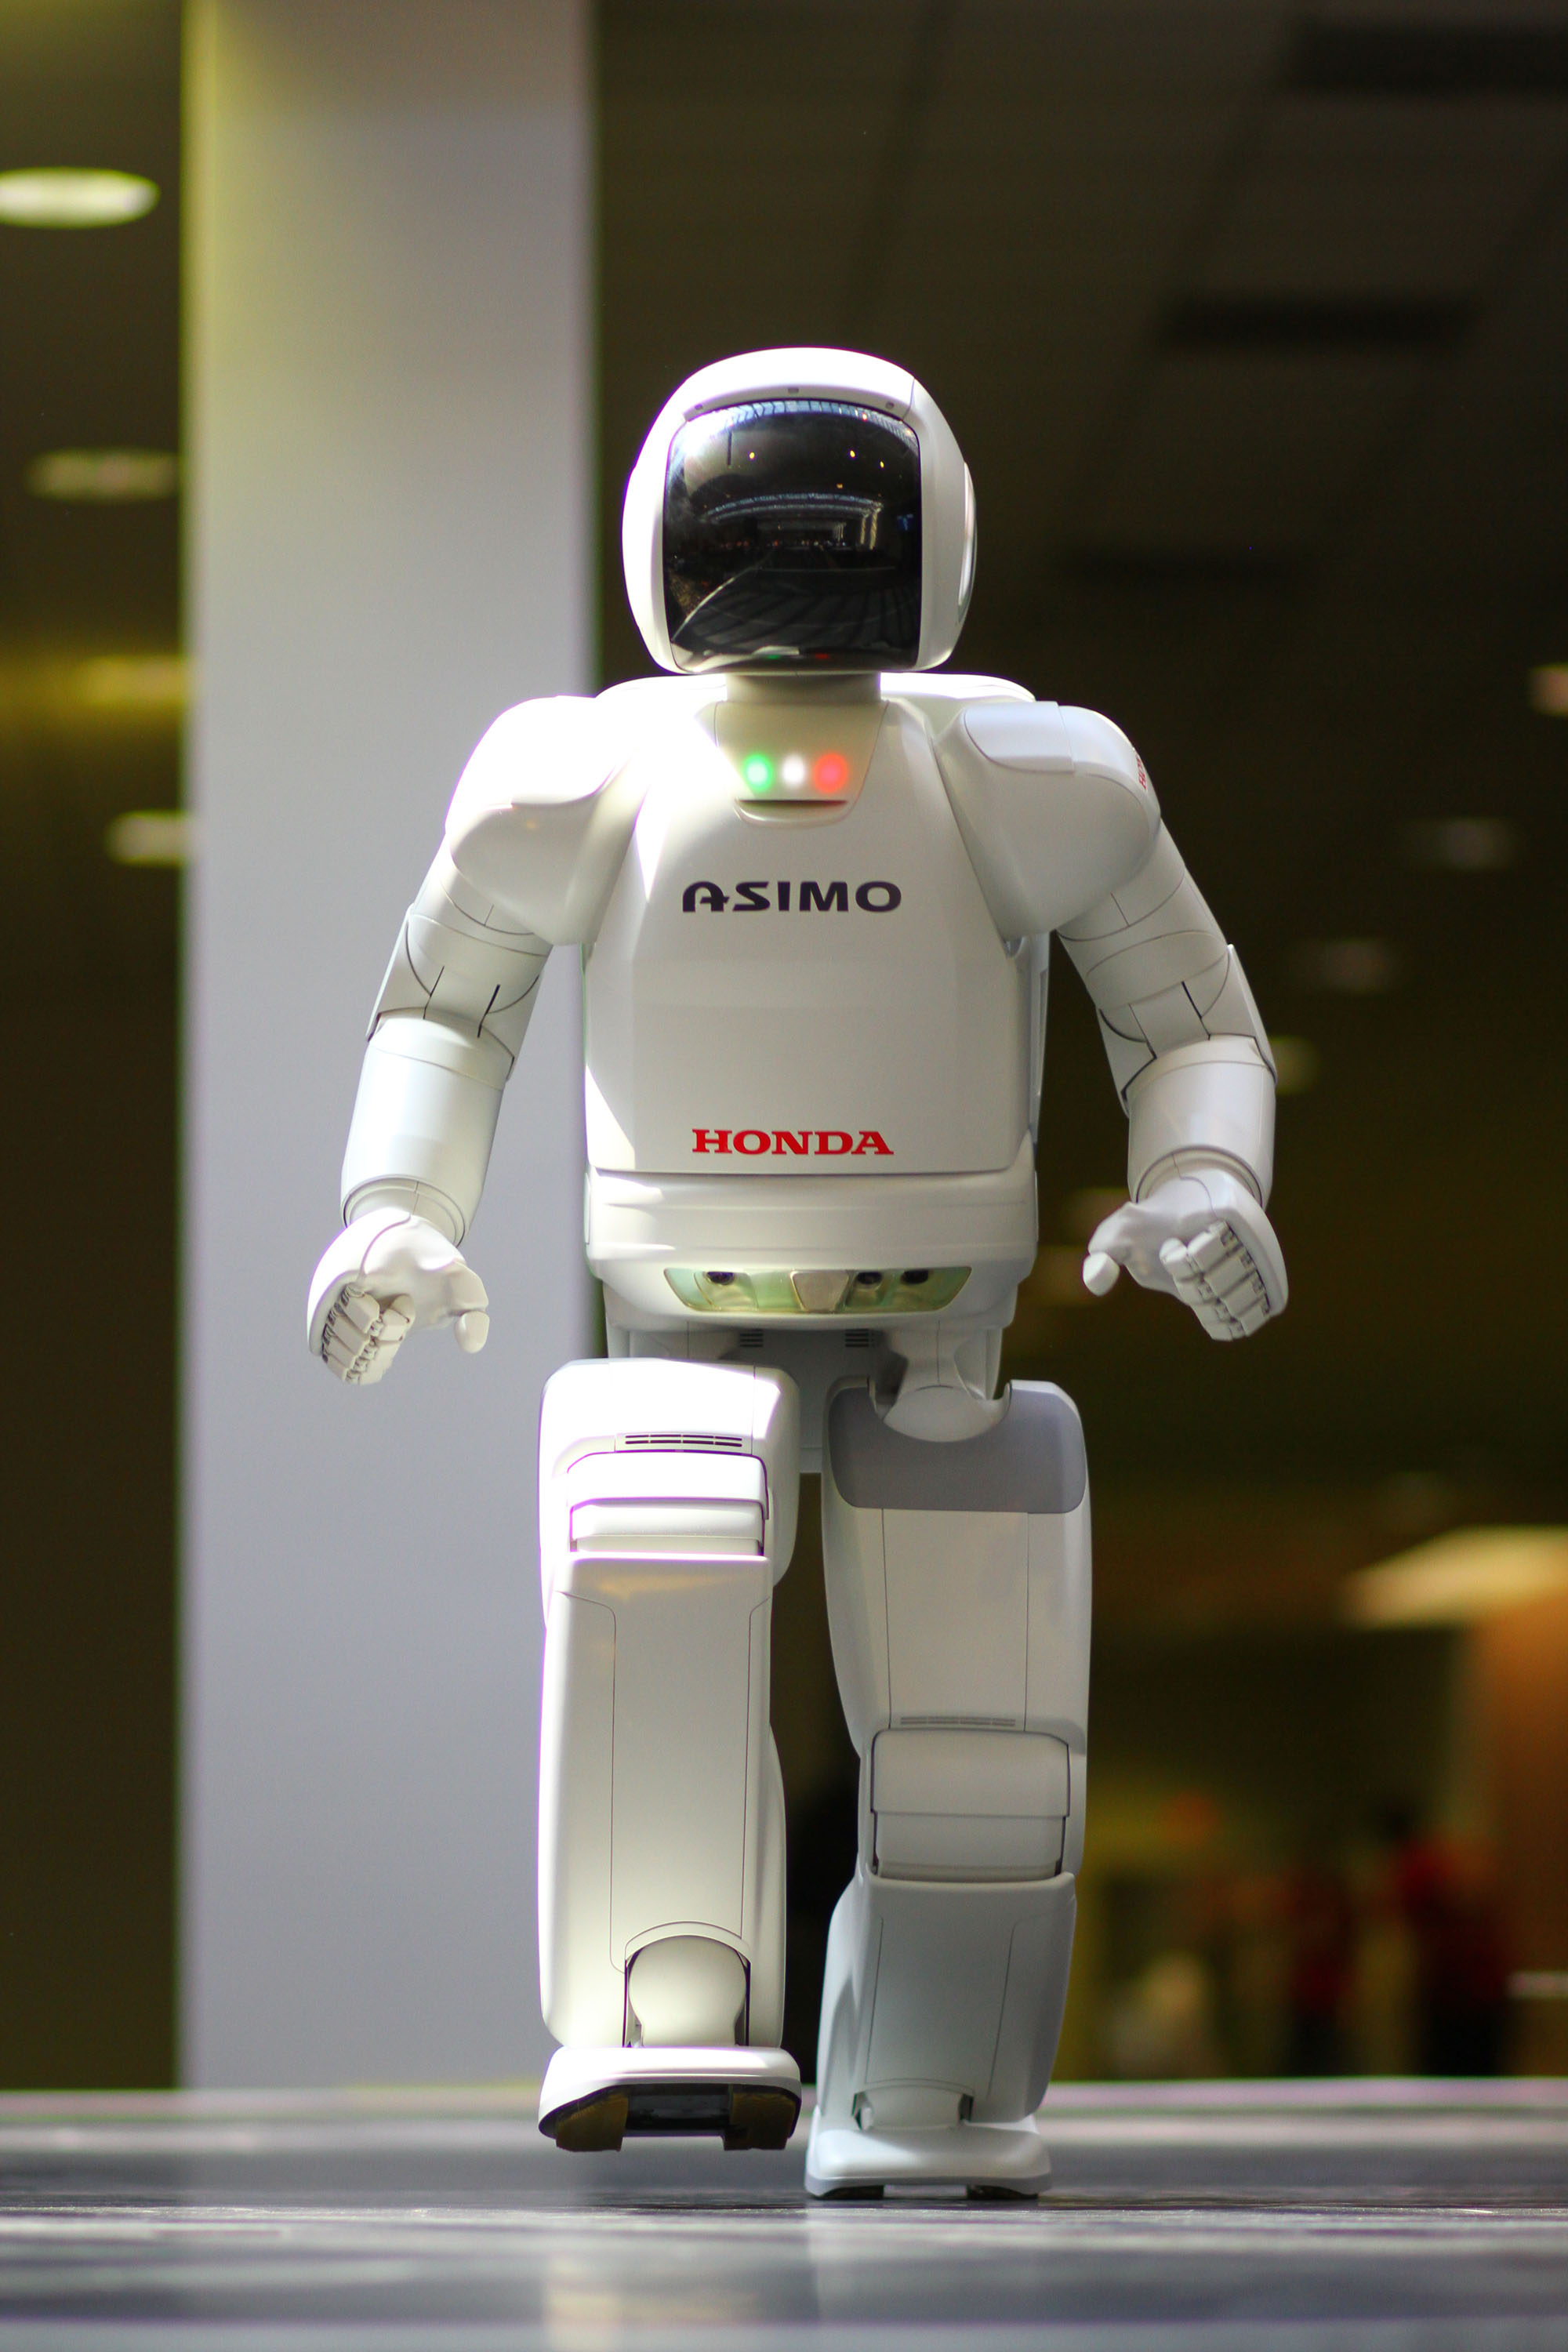
\includegraphics[width=\textwidth]{figures/ASIMO.jpg}
    \caption{}
    \label{fig:asimo}
  \end{subfigure}
  \caption{WABOT-1 \cite{Kato1973TheWABOT1AI} on the left, the first 
      anthropomorphic robot. ASIMO \cite{Sakagami2002TheIntelligentASIMO} on
      the right.}
\end{figure}

\begin{figure}
  \centering
  \begin{subfigure}[b]{0.4\textwidth}
    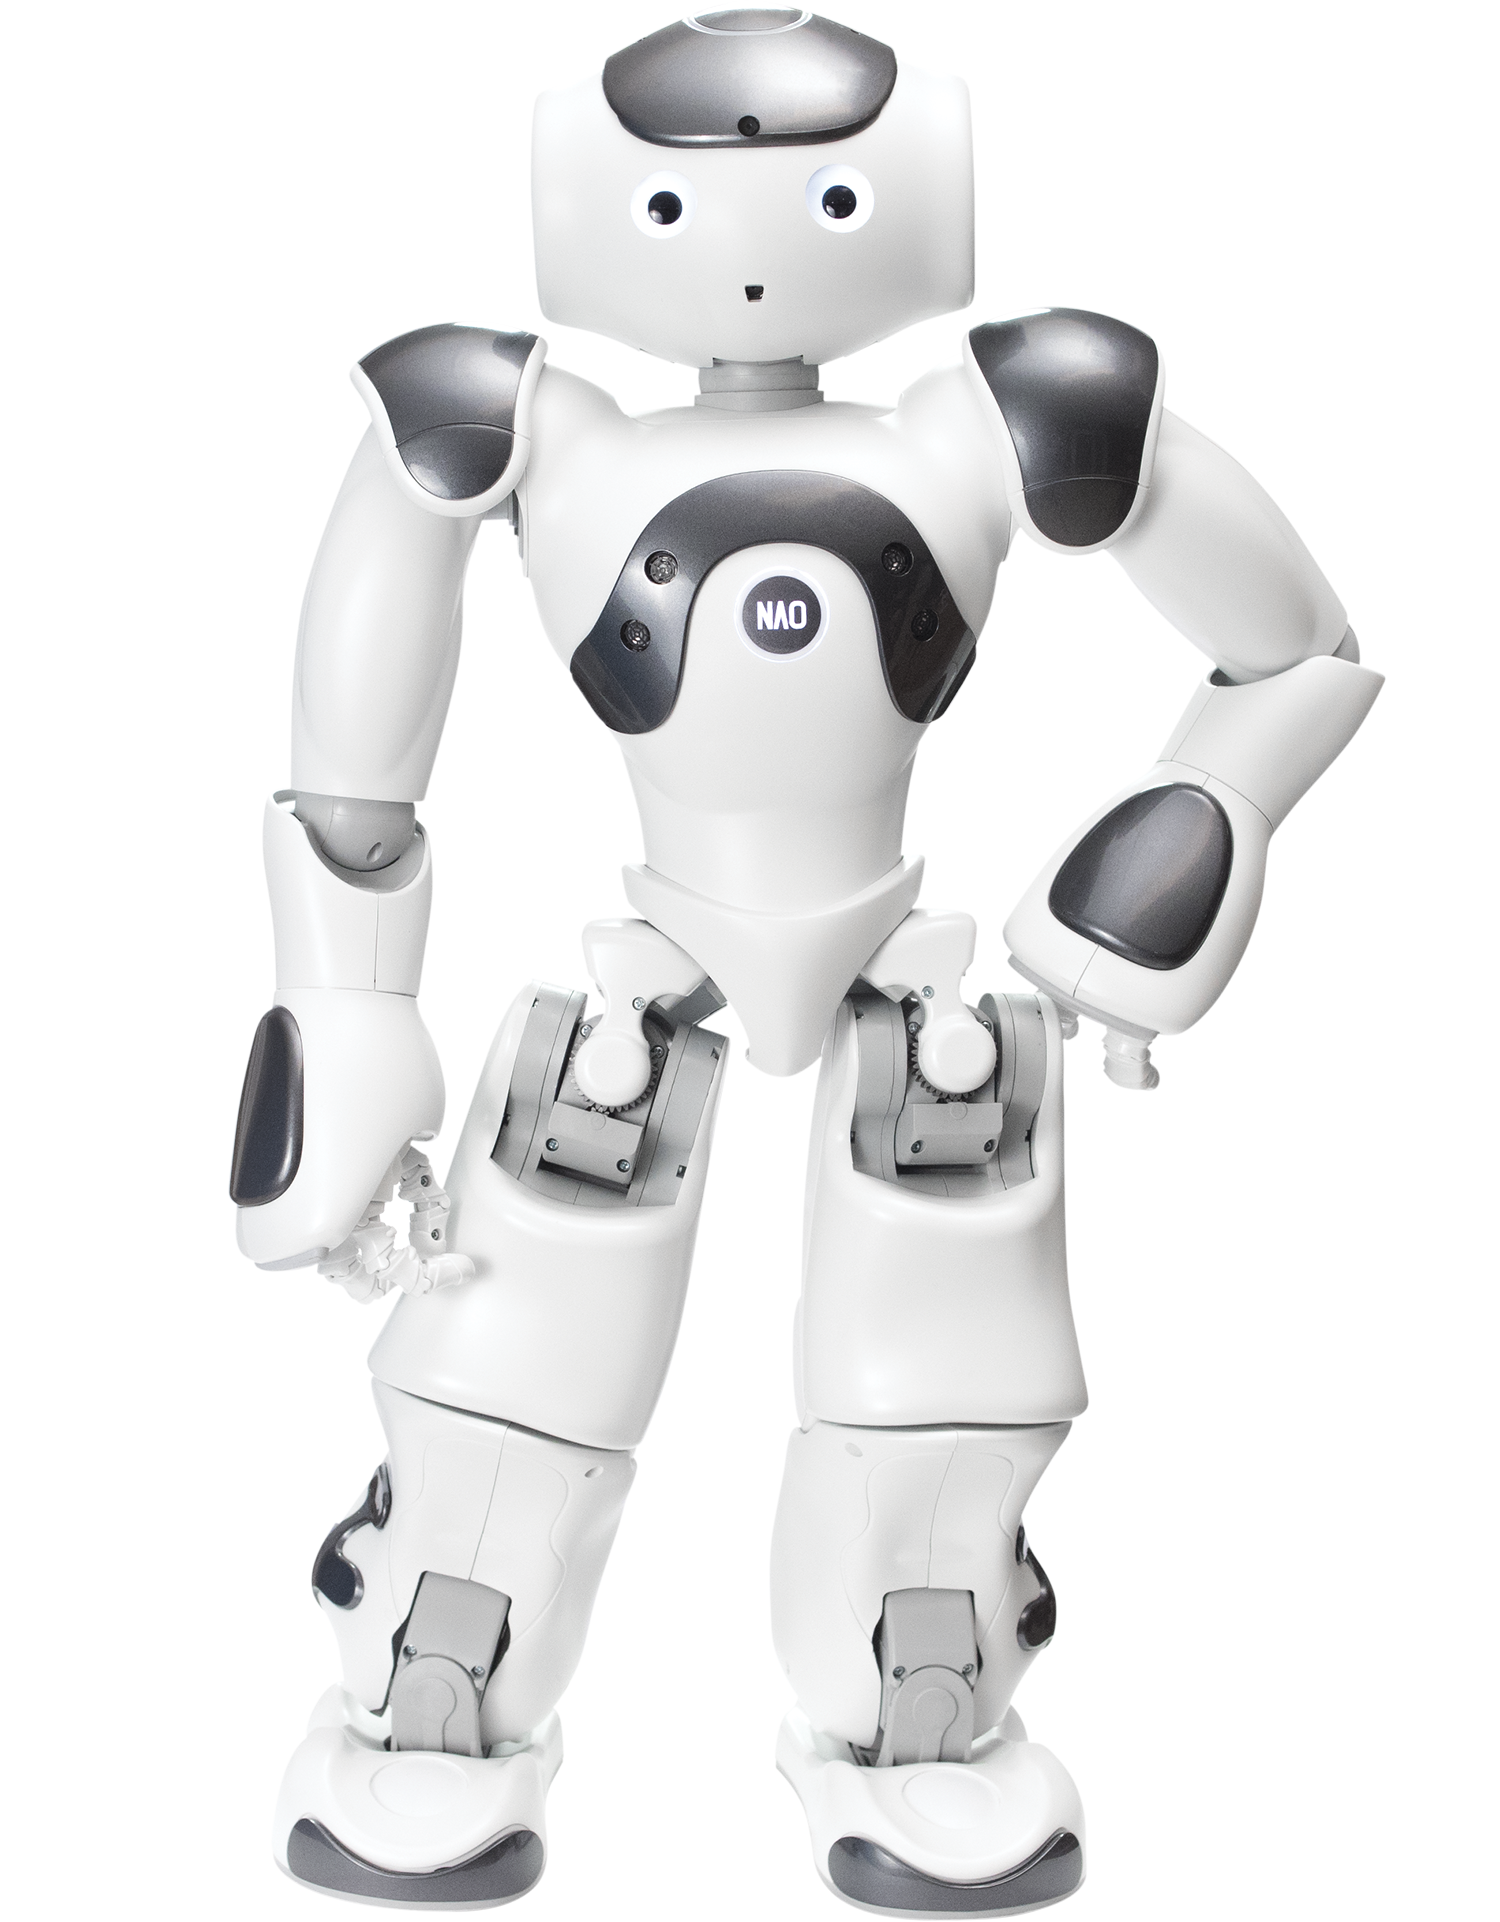
\includegraphics[width=\textwidth]{figures/NAO-v6.png}
    \caption{}
    \label{fig:nao-v6}
  \end{subfigure}
  \begin{subfigure}[b]{0.4\textwidth}
    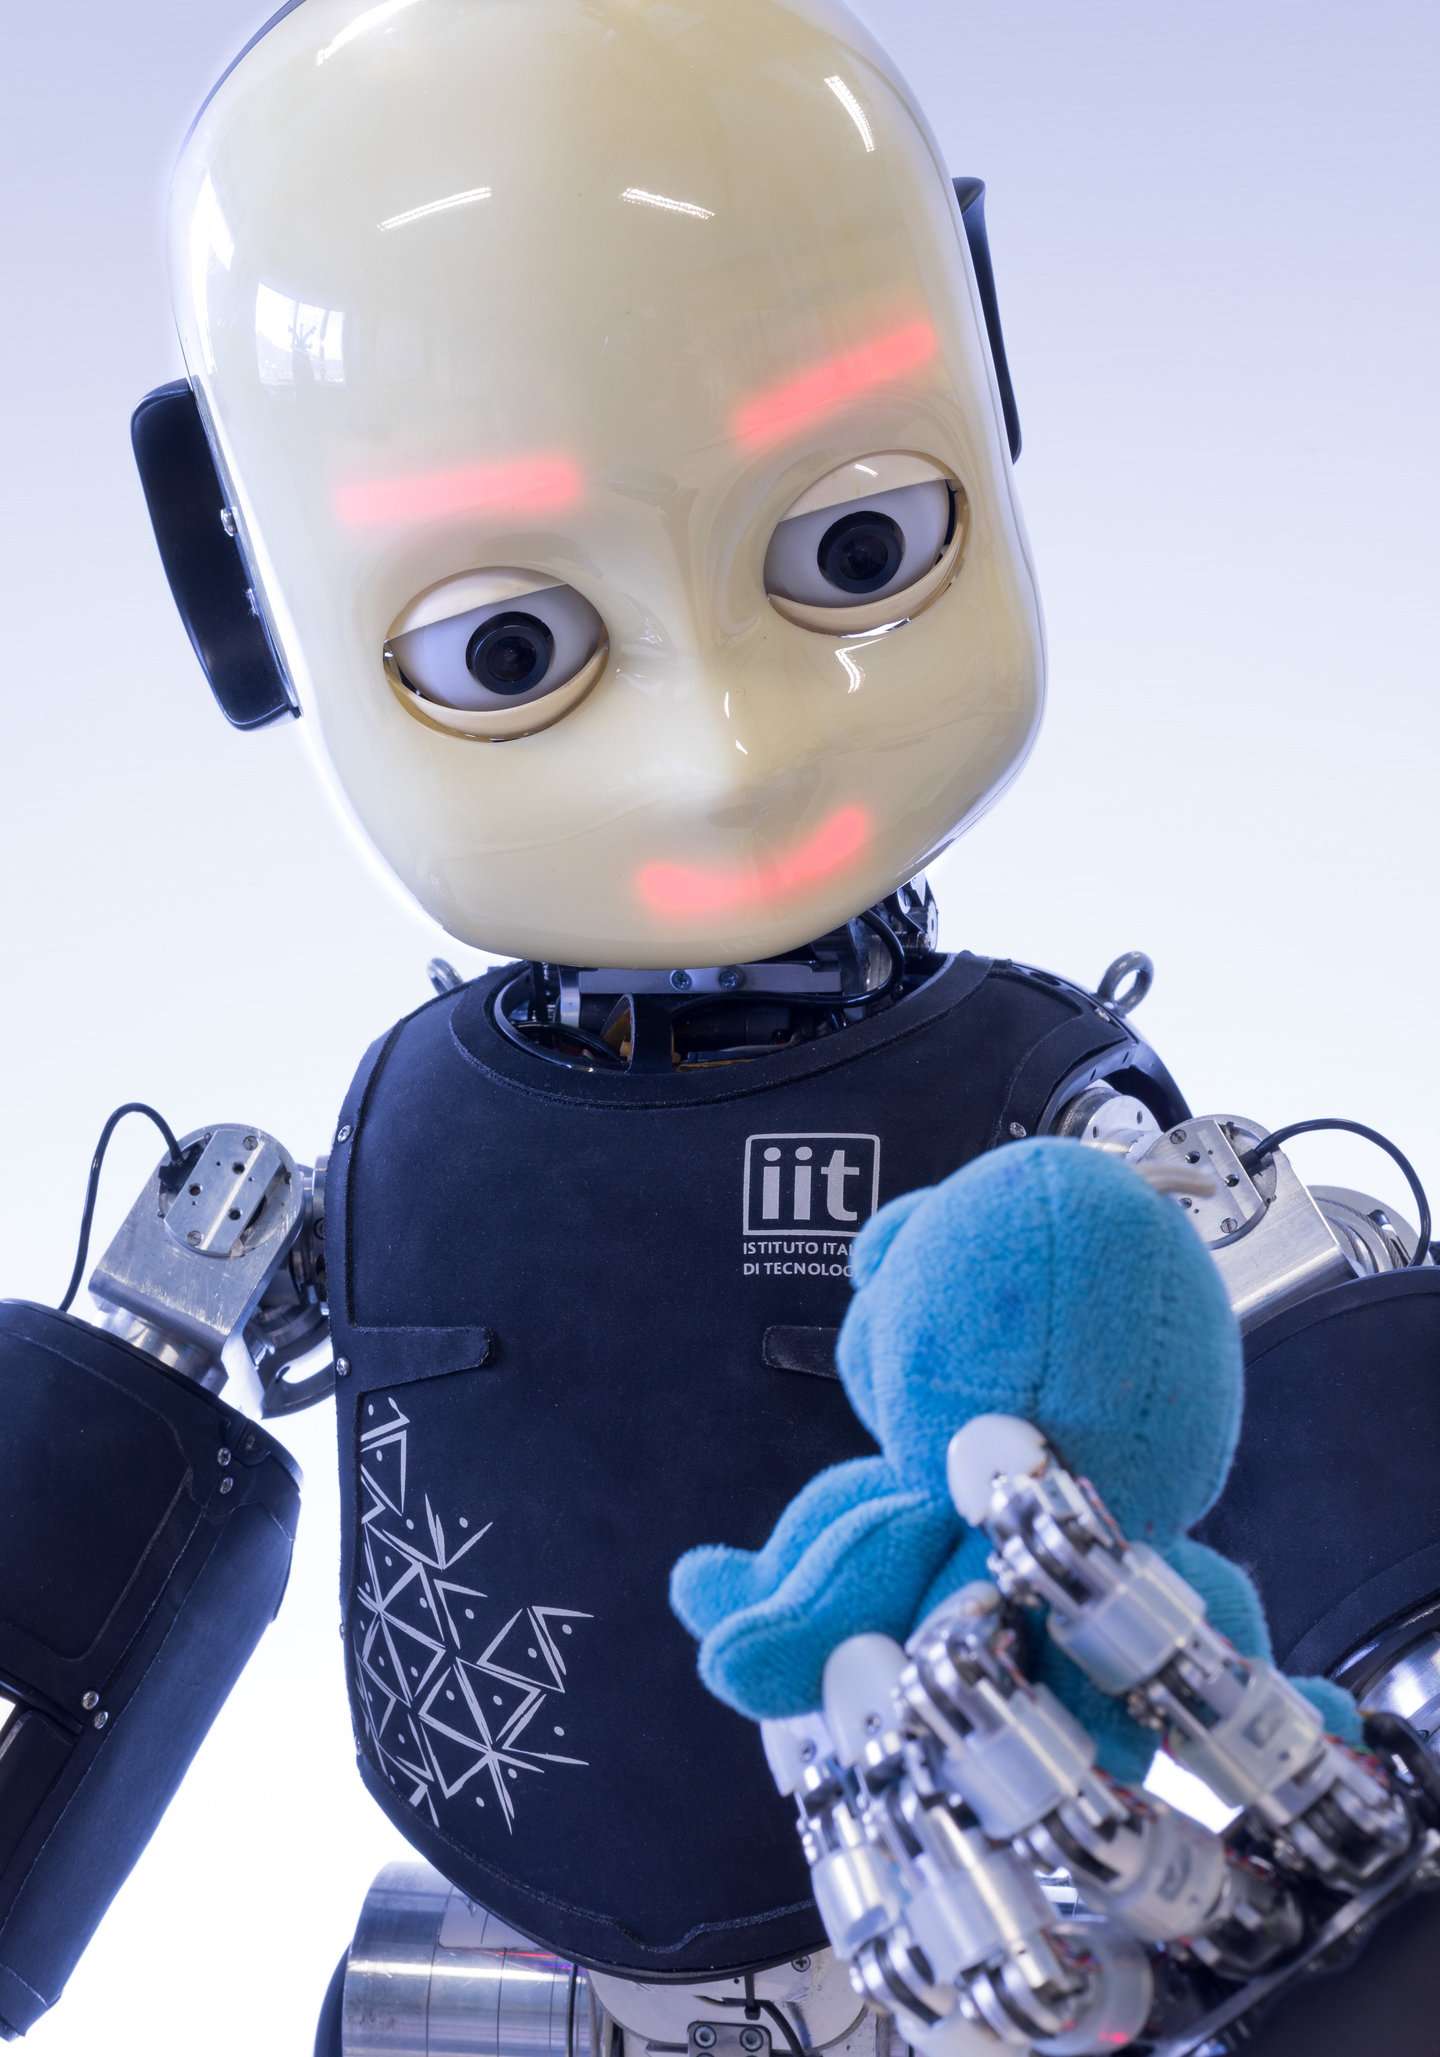
\includegraphics[width=\textwidth]{figures/iCub.jpeg}
    \caption{}
    \label{fig:iCub}
  \end{subfigure}
  \caption{NAO v6 \cite{NAOdesign} on the left, used in RoboCup Standard 
      Platform League. iCub \cite{Sandini2007iCub} on the right, a cognitive 
      robotics research platform.}
\end{figure}

\begin{figure}
  \centering
  \begin{subfigure}[b]{0.4\textwidth}
    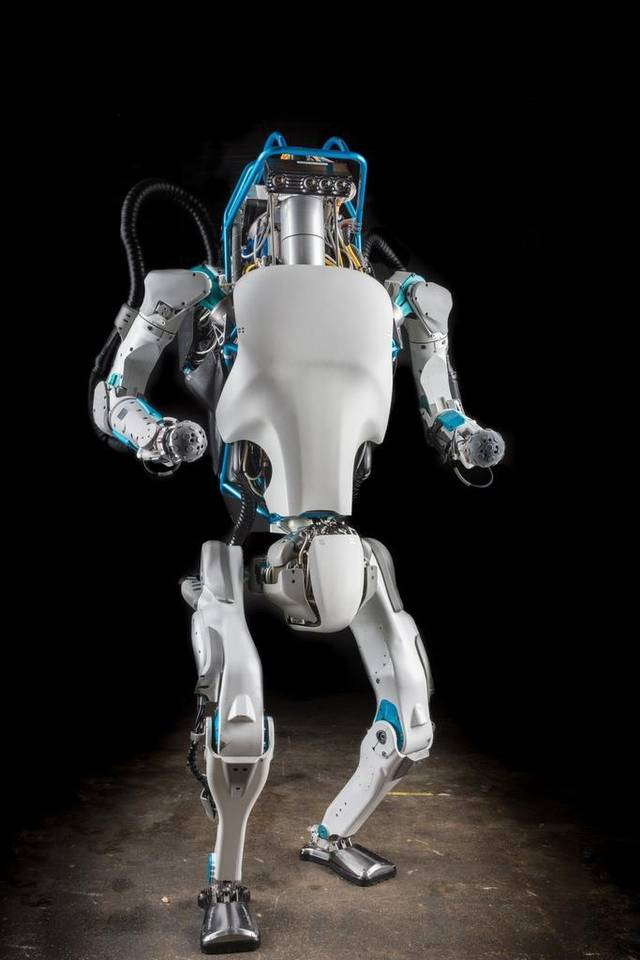
\includegraphics[width=\textwidth]{figures/ATLAS.jpg}
    \caption{}
    \label{fig:atlas}
  \end{subfigure}
  \begin{subfigure}[b]{0.4\textwidth}
    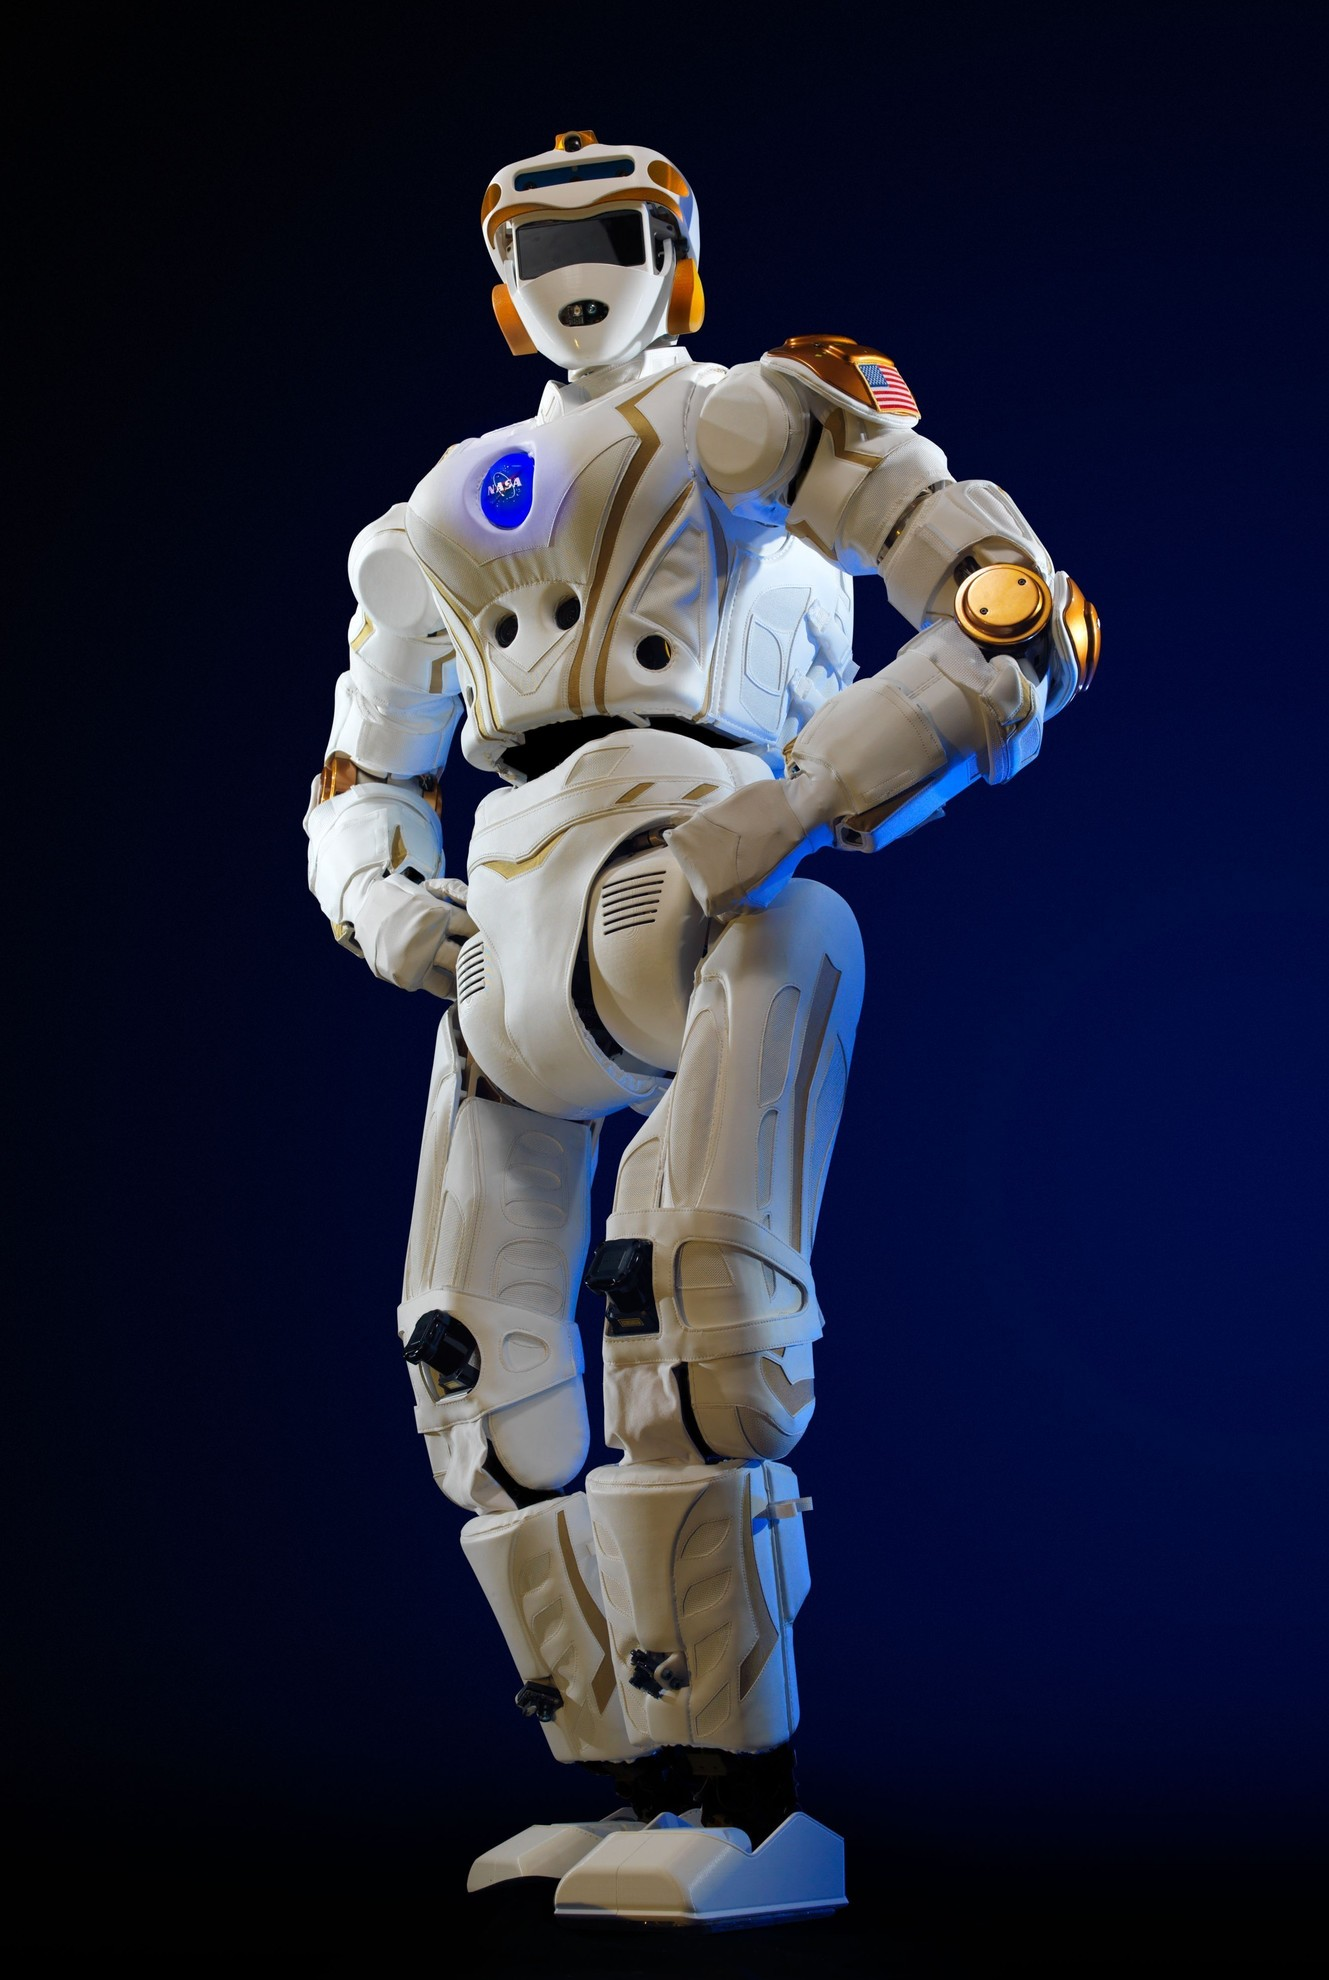
\includegraphics[width=\textwidth]{figures/NASA-Valkyrie.jpeg}
    \caption{}
    \label{fig:valkyrie}
  \end{subfigure}
  \caption{ATLAS, on the left, and Valkyrie \cite{Radford2015Valkyrie}, on the 
      right, have been developed with the purpose of advancing rescue operations
      and space exploration missions.}
\end{figure}

\begin{figure}
  \centering
  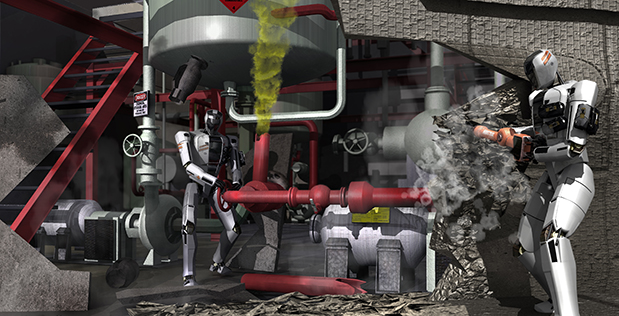
\includegraphics[width=\textwidth]{figures/DARPARoboticsChallenge.jpg}
  \caption{Typical scenarios described by DARPA Robotics Challenge
      \cite{Atkenson2018DARPARoboticsChallengeFinals}, where the human 
      intervention is dangerous and could put at risk life of rescuers.}
  \label{fig:drc}
\end{figure}

Unlike other traditional robots, such as industrial manipulators (Fig.
\ref{fig:kuka-lwr-IV}) or wheeled mobile robots
(Fig. \ref{fig:ethz-heap-excavator}),
humanoid robots are capable of handling a larger number of scenarios, such as 
rescue operations and space exploration, described above, but also classical
ones that are part of our daily life, namely all the activities that humans
perform during the day, that go from the manipulation of simple objects to
communication. Humanoids are able to cover all these tasks because of their
similarity to the humans, allowing them to interact with our environment and 
with other people. In order to successfully perform these tasks, humanoid 
robots need to properly move inside complex environments.
\begin{figure}
  \centering
  \begin{subfigure}[b]{0.3\textwidth}
    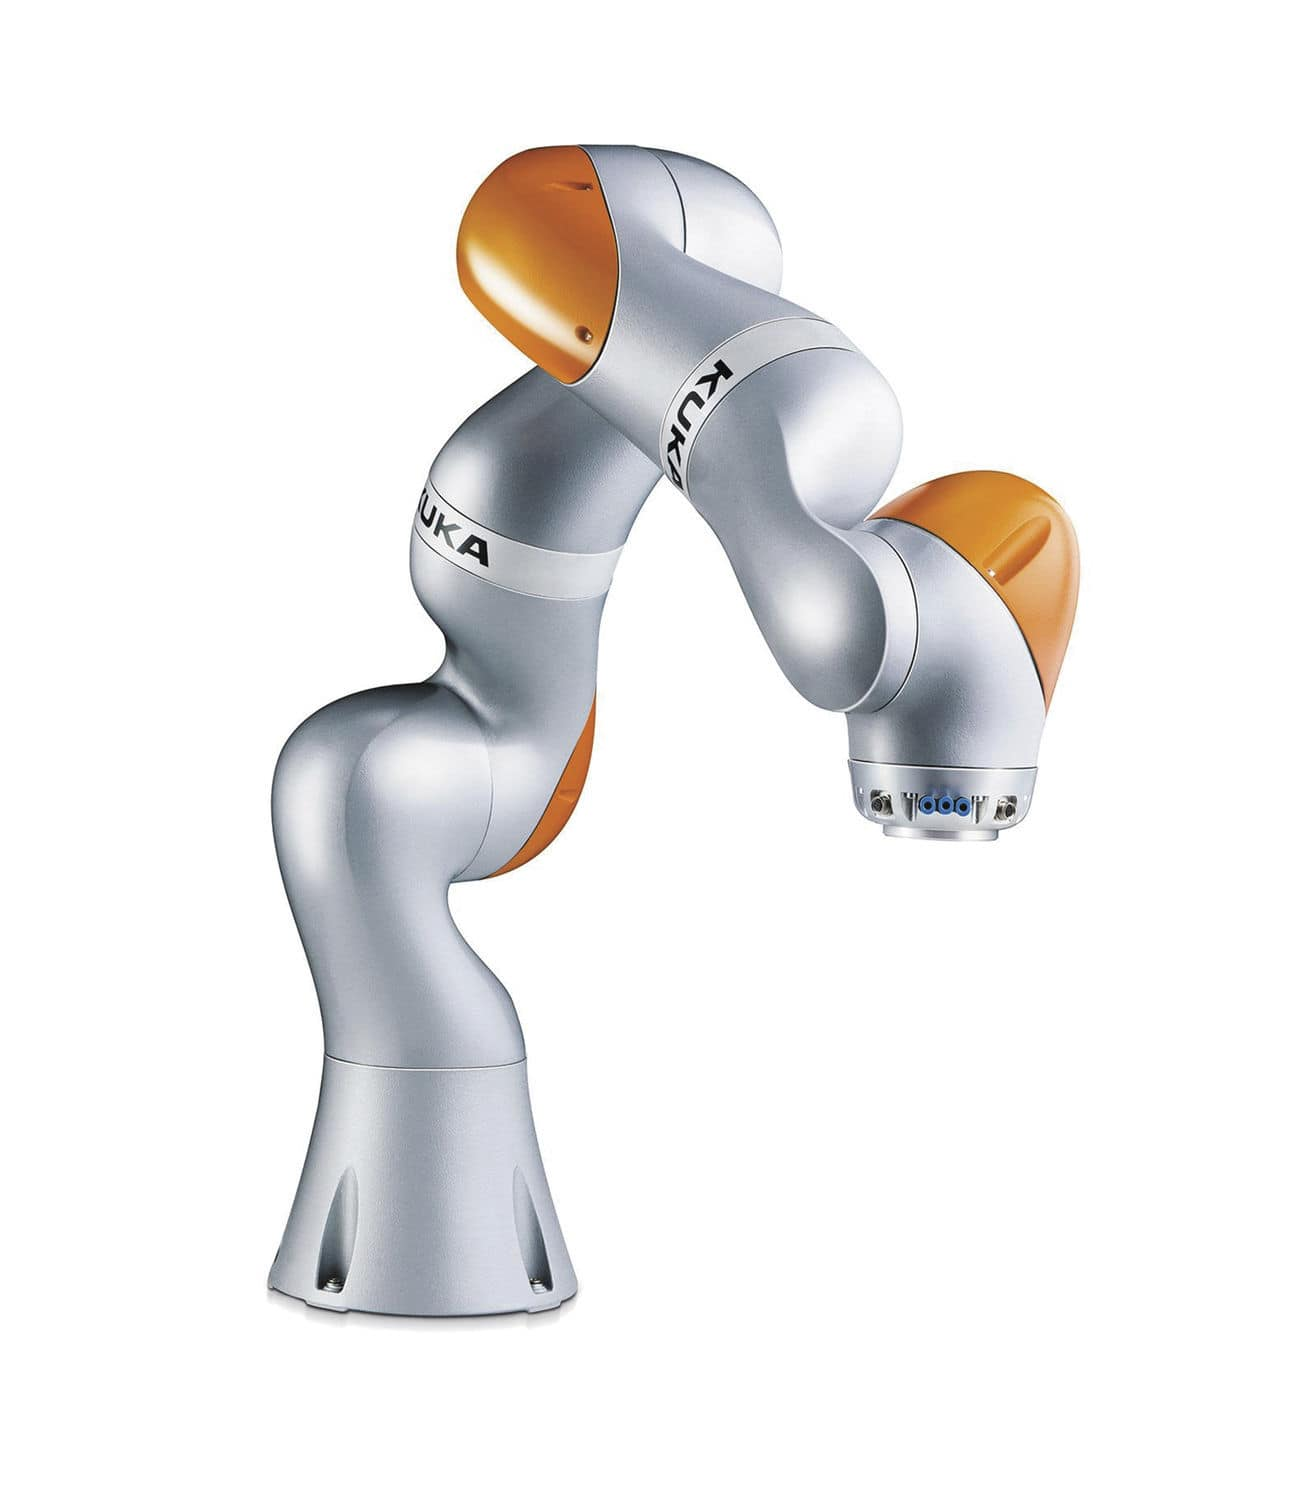
\includegraphics[width=\textwidth]{figures/kuka-lwr-IV.jpg}
    \caption{}
    \label{fig:kuka-lwr-IV}
  \end{subfigure}
  \begin{subfigure}[b]{0.6\textwidth}
    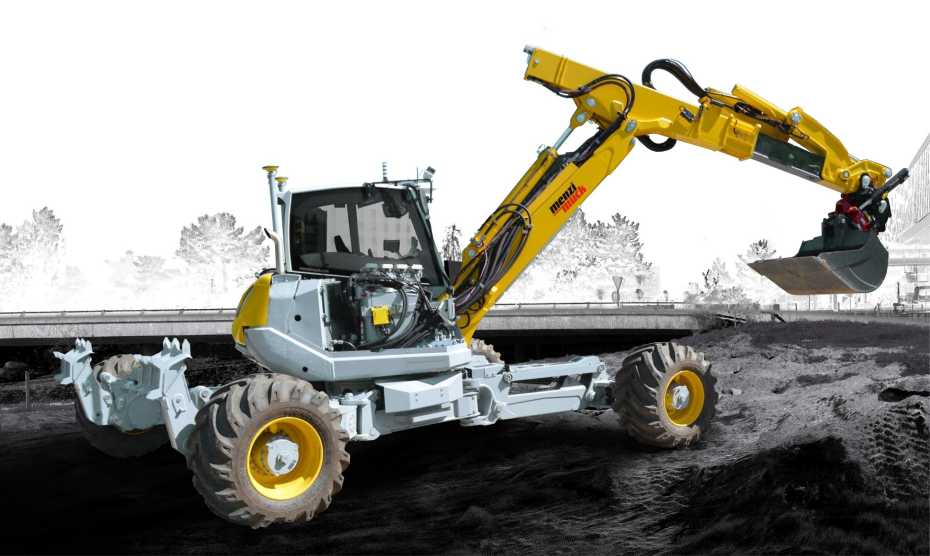
\includegraphics[width=\textwidth]{figures/ethz-heap-excavator.jpg}
    \caption{}
    \label{fig:ethz-heap-excavator}
  \end{subfigure}
  \caption{On the left, KUKA LWR \cite{Gaz2014KUKALWR}, a famous industrial
      manipulator. On the right, HEAP \cite{Hutter2015WalkingExcavators},
      an autonomous hydraulic walking excavator.}
\end{figure}


\section{Legged Robot Locomotion}
The problem of humanoid robot locomotion, or more in general legged robot 
locomotion, consists in developing algorithms that allow humanoids to 
safely move inside an environment. In order to successfully perform this task,
a humanoid robot needs to understand the structure of the
surrounding environment and its configuration with respect to the world.
Once a representation of the 
environment has been created, the robot needs to plan its motion in order to
move without colliding with obstacles and without compromizing its integrity.
The plan needs to be correctly executed, keeping the robot in equilibrium,
avoiding falls and collisions. These are the most important characteristics
that allow a sound generation of humanoid gaits.

A typical humanoid robot locomotion pipeline consists in a localization module,
that determines the configuration of the robot with respect to the world; a 
mapping module, that determines a representation of the world that can be used 
efficiently by the robot; a planning module, that uses the configuration of 
the robot and the configuration of world in order to generate a plan that 
allows the humanoid to move from its configuration to a specified one;
a control module, that guarantees that the motion generated by the planning
module is correctly executed.

\subsection{Localization and Mapping}
The purpose of localization is to provide the pose of the robot with respect
to the world. Localizing accurately is of fundamental importance in order to
guarantee that the robot behaves in a correct way during the execution of its
tasks. The introduction of advanced sensors, such as IMU (accelerometer,
gyroscope), RGB-D cameras, LIDAR and sonars, makes it possible to observe
the surrouding environment and consequently to localize the robot. Many
different techniques can be used for robot localization, such as
particle filters \cite{Hornung2010HumanoidRobotLocalization}, Extended
Kalman Filters \cite{Oriolo2015HumanoidOdometricLocalization} and V-SLAM
\cite{Tanguy2019MPCWithDenseVisualSLAM}.

The purpose of mapping is to provide a representation of the environment that
can be used to make the robot navigate. A mapping program should be able to
recreate the world with enough details to make locomotion safe. Moreover,
the implementation should be efficient enough to provide the map in real-time.
These characteristics are essential to make the robot truly autonomous.
The most used representations are elevation maps
\cite{Siciliano2016HandbookRobotics}, which store the map as a grid such that
for each point $(x, y, z)$ on the surface there exists a cell $(x, y)$ in the 
grid that stores the corresponding height $z$, and OctoMaps
\cite{Hornung2013OctoMap}, a representation based on octrees that efficiently
determines if a point in space is occupied or free.

\subsection{Planning}
A planning algorithm consists in generating a sequence of motion primitives
that allow a robot to move from its current location to a desired one. In
order to generate this sequence, the planner needs a map that represents
the environment. Regarding humanoid robots, most famous planning approaches
generate sequence of consecutive footsteps that the robot should follow in order
to reach the desired goal. There exists a variety of techniques based on
heuristic search, such as A* \cite{Chestnutt2005FootstepPlanningASIMO}, that
provides an optimal plan, and ARA*
\cite{Hornung2012AnytimeSearchBasedFootstepPlanning}, that provides a suboptimal
plan but is faster than the previous method. Other techniques are 
optimization-based, i.e. they generate a plan by solving an optimization 
problem, such as \cite{Herdt2010OnlineWalkingMotionGenerationWithAFSP}, that
solves a quadratic programming (QP) problem, and
\cite{Deits2015FootstepPlanningUnevenTerrainMIQCQP}, that solves a 
mixed-integer quadratically-constrained quadratic programming (MIQCQP) problem.
Another family of algorithms are sampling-based and generates a tree of 
footstep configuration randomly, for example by using Rapidly-Exploring
Random Trees (RRTs) \cite{ECC19}.

\subsection{Control}
Once a footstep plan has been generated, the robot needs to execute it
without falling. Here, a motion model is needed to describe the behaviour of 
the system. Usually, since the dynamics of the humanoid robots is complex,
a simplified once is used, such as the dynamics of the Linear Inverted 
Pendulum (LIP) \cite{Kajita1991StudyOD}. The introduction of the LIP allowed
the development of control modules that generate humanoid gaits. The most 
famous works include the Preview Control \cite{Kajita2003BipedWP}, which
uses a dynamic extension of the Cart-Table model solving a LQR problem;
the Model Predictive Control (MPC) \cite{wieber:inria-00390462},
which constraints ZMP to keep the
robot balanced, solving a QP problem; the Intrinsically-Stable MPC (IS-MPC)
\cite{DBLP:conf/humanoids/SciancaCSLO16}, which guarantees to produce
stable CoM trajectories by constraining both the ZMP and the unstable mode
of the LIP. After the generation of a desired trajectory, a kinematic 
controller is responsible for execution of the motion task at the lowest
level.


\section{Thesis Overview}
The goal of the thesis is that of studying humanoid robot locomotion in a
world known as \textit{World of Stairs}, a particular uneven ground composed
by horizontal patches located at different heights \cite{ECC19}. The idea is
that of making NAO humanoid robot walk in a complex scenario, making it
climb stairs and avoid obstacles. The robot needs to autonomously perceive
the surrouding world, create a representation of the environment, generate
a plan that allows the robot to safely reach a specified region of the world
and correctly execute the motion. The robot has been equipped with an RGB-D
sensor, which has been mounted on its head.

The approach is to use the depth sensor of the camera in order to generate
an elevation map of the environment. To do this, \texttt{elevation\_mapping}
\cite{Fankhauser2018ProbabilisticTerrainMapping} has been used. Once the 
map has been created, a footstep planner based on RRT \cite{ECC19}
generates a sequence
of footsteps with the respective swing foot trajectories (taking into account
collisions and the limitations of the robot) that allow
the robot to reach a desired final position. To guarantee that the motion
is properly executed, a Variable-Height CoM IS-MPC \cite{SYROCO18} is used to
generate a trajectory of the CoM of the robot. In the end, a pseudo-inverse
based kinematic controller computes the joint commands of the robot needed to
execute the motion. Fig. \ref{fig:block-scheme} illustrates a block scheme
of the described approach.

\begin{figure}
  \centering
  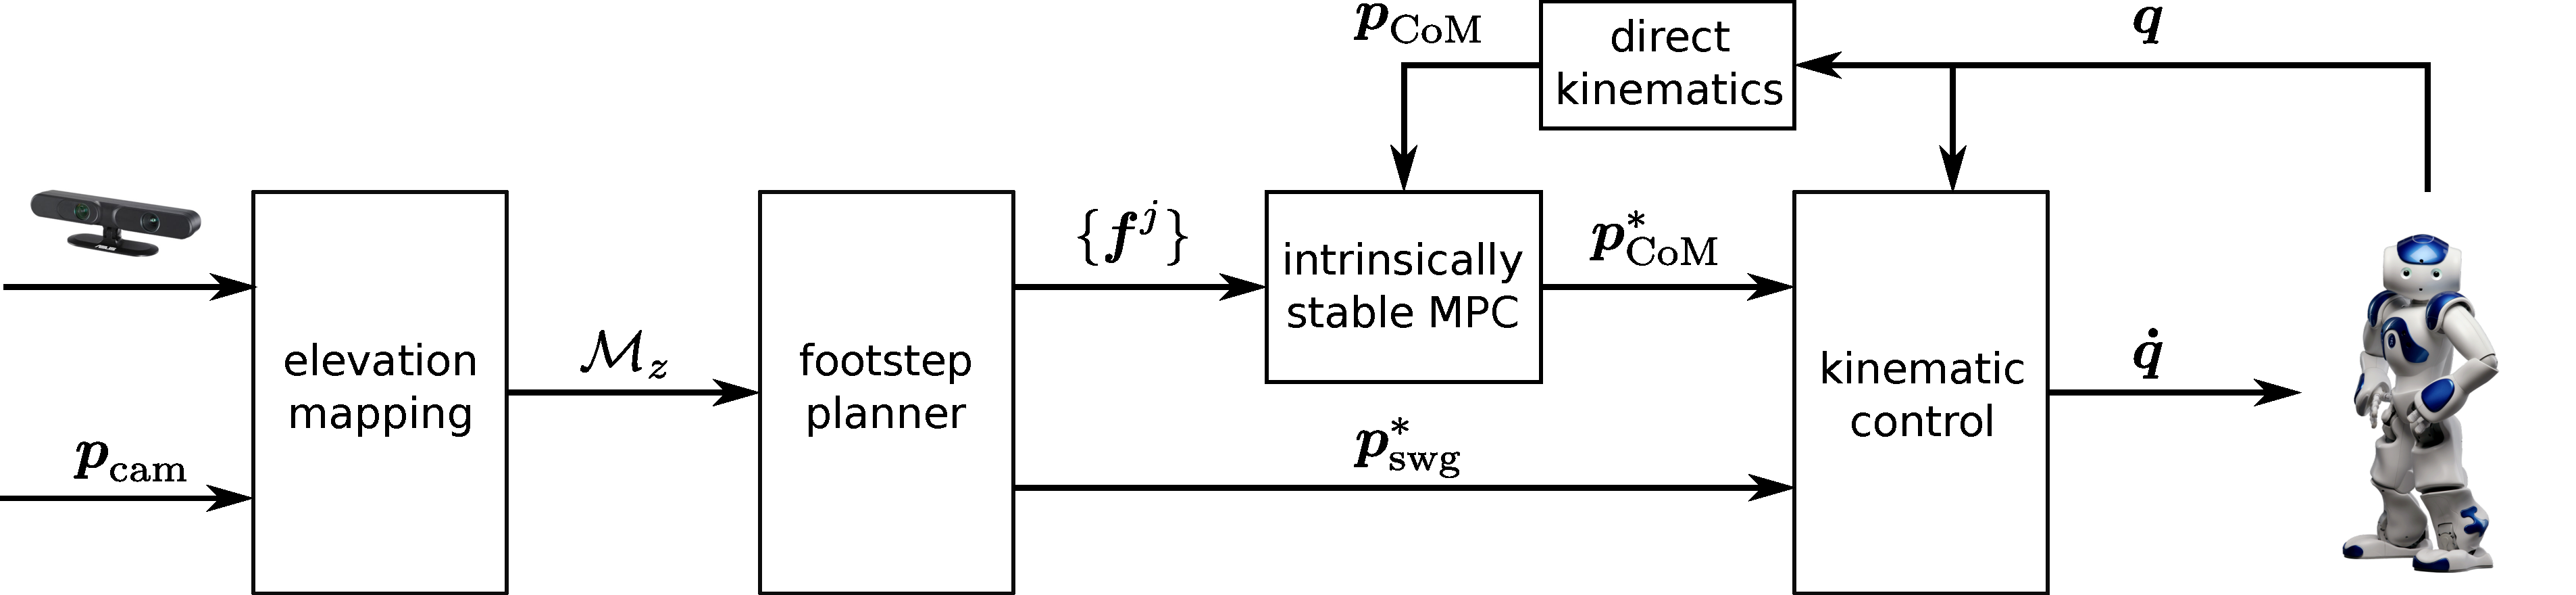
\includegraphics[width=\textwidth]{figures/BlockScheme.pdf}
  \caption{Block scheme of the approach.}
  \label{fig:block-scheme}
\end{figure}

This thesis extends \cite{ECC19}, providing an implementation of the
Variable-Height CoM IS-MPC for a real humanoid robot (NAO), extending the 
RRT-based footstep planner to work in a real environment with NAO and 
introducing \texttt{elevation\_mapping} (directly extending the block scheme
of \cite{ECC19}) in order to generate an elevation map of the terrain,
making NAO able to execute gaits in a \textit{World of Stairs} unknown
environments.

Chapter \ref{ch:elevation-map-generation} introduces
\texttt{elevation\_mapping}, describing the framework and its integration with
the camera, the planner and the robot. Chapter
\ref{ch:rrt-based-footstep-planning} describes the RRT-based footstep planner
introduced in \cite{ECC19}, formulating the problem, the algorithm and
discussing its integration with NAO. Chapter \ref{ch:vh-com-is-mpc} describes
the Variable-Height CoM IS-MPC and the implementation on the BHuman framework
\cite{BHumanCodeRelease2018}. Chapter \ref{ch:experiments} presents the
experiments performed on the robot in different scenarios, using the three
modules described in the previous three chapters. Chapter \ref{ch:conclusion}
concludes the thesis by summarizing the obtained results and discussing
future works.

